\documentclass[11pt,a4paper]{article}
\usepackage[T1]{fontenc}
\usepackage[utf8]{inputenc}
\usepackage{lmodern}
\usepackage[margin=22mm,headheight=16pt]{geometry}
\usepackage{amsmath,amssymb,graphicx,array,longtable,booktabs}
\usepackage{microtype,xcolor,hyperref,xurl,fancyhdr}
\definecolor{Navy}{HTML}{17324D}
\definecolor{Teal}{HTML}{087F8C}
\definecolor{Gold}{HTML}{B88128}
\hypersetup{colorlinks=true,linkcolor=Navy,urlcolor=Teal,bookmarksnumbered=true,hypertexnames=false}
\setlength{\parindent}{0pt}
\setlength{\parskip}{6pt}
\setlength{\emergencystretch}{4em}
\setcounter{tocdepth}{1}
\pagestyle{fancy}\fancyhf{}
\fancyfoot[R]{\small\thepage}
\fancyfoot[L]{\small\sffamily Sharif University of Technology}
\renewcommand{\headrulewidth}{0.3pt}
\makeatletter
\renewcommand\section{\@startsection{section}{1}{\z@}{-3.2ex plus -1ex minus -.2ex}{1.6ex plus .2ex}{\normalfont\Large\sffamily\bfseries\color{Navy}}}
\renewcommand\subsection{\@startsection{subsection}{2}{\z@}{-2.5ex plus -1ex minus -.2ex}{1.2ex plus .2ex}{\normalfont\large\sffamily\bfseries\color{Teal}}}
\makeatother
\fancyhead[L]{\small\sffamily\color{Navy}Reza Sanaee Nezhad}\fancyhead[R]{\small\sffamily\color{Teal}Technical Report}\begin{document}
\begin{titlepage}\centering\vspace*{7mm}

\includegraphics[width=31mm]{assets/sharif_emblem_en.png}\par\vspace{5mm}
{\Large\sffamily\bfseries\color{Navy}SHARIF UNIVERSITY OF TECHNOLOGY\par}
\vspace{2mm}{\sffamily Department of Electrical Engineering\par}
\vspace{17mm}{\color{Teal}\rule{\linewidth}{1.4pt}}\par\vspace{6mm}
{\large\sffamily\color{Teal}TECHNICAL REPORT\par}
\vspace{8mm}{\huge\sffamily\bfseries\color{Navy}Periodic Real-Time Scheduling Simulator: RM, DM, and EDF\par}
\vspace{9mm}{\color{Gold}\rule{45mm}{1pt}}\par\vfill
\begin{minipage}{.88\linewidth}{\sffamily\color{Teal}AUTHOR}\par{\Large\sffamily Reza Sanaee Nezhad}\par Student ID: 401101502\par\vspace{7mm}
{\sffamily\color{Teal}INSTRUCTOR / INSTRUCTORS}\par
Dr Iman Gholampour\par\vspace{7mm}
{\sffamily\color{Teal}ACADEMIC CONTEXT}\par
Embedded Systems\par\end{minipage}\vfill
\end{titlepage}
\tableofcontents\clearpage
\section{Embedded architectures}

A single-processor system simplifies implementation, communication, and scheduling, and can suit household controls, simple IoT sensors, and small controllers. Its limited compute capacity makes substantial parallel work difficult. Execution variability and power consumption depend on interrupts, caches, peripherals, clock settings, and workload. Multicore architectures allow concurrent computation and are useful for image processing and advanced driver-assistance workloads. Shared-memory synchronization, inter-core communication, cache interference, and scheduling complicate analysis. More active cores can increase power, but an energy comparison requires a measured workload and power policy. A system-on-chip integrates processors, interfaces, peripherals, and possibly accelerators and memory on one device. Integration reduces board size and enables close coupling. Custom chip design can have substantial nonrecurring engineering cost and limited hardware upgradeability;\allowbreak{} purchasing an existing SoC is a different cost model. Smartphones, networking equipment, and drones illustrate integrated platforms. "SoC" describes integration, so it can coexist with either a single-core or multicore processor.

\[ U=\sum_i C_i/T_i,\qquad R_i=C_i+\sum_{j\in hp(i)}\lceil R_i/T_j\rceil C_j. \]
\section{Real-time versus general-purpose operating systems}

An RTOS is designed to support bounded, analyzable response times under specified assumptions. Priority-based preemption is common, but an RTOS does not automatically make every application meet its deadlines. General-purpose systems balance throughput, fairness, responsiveness, and many concurrent services, which can make worst-case response harder to bound. Fixed-size memory pools and avoidance of demand paging help limit timing variability. General-purpose virtual-memory operations can introduce page faults and reclamation delays. Real-time designs also minimize and bound interrupt latency;\allowbreak{} hardware, interrupt priorities, drivers, critical sections, and configuration affect that bound. These distinctions motivate explicit timing analysis rather than inferring guarantees from an operating-system label.

\section{Priority inversion and resource protocols}

Priority inversion occurs when a high-priority job waits for a lock held by a low-priority job, while a medium-priority job preempts the lock holder and prolongs the high-priority wait. Priority inheritance temporarily boosts the lock holder to the waiting job's priority so it can release the resource sooner. Chained dependencies and lock discipline still matter. Ceiling protocols assign each resource a ceiling based on the highest-priority task that can use it. Immediate priority elevation on locking corresponds to an immediate-ceiling formulation. Under their specified assumptions, ceiling protocols can bound blocking and prevent certain deadlock patterns. Priority inheritance and the different ceiling formulations must not be treated as interchangeable or unconditional deadlock cures.

\section{Hard and soft deadlines}

A hard real-time requirement treats exceeding a deadline as unacceptable for the function being assured. Automotive braking and airbag-control functions illustrate safety-critical timing needs, although the exact permissible interval depends on the specification and is not established by the report's illustrative 100-ms number. Soft real-time services tolerate occasional lateness with degraded quality, as in video streaming or online games. A missed deadline does not necessarily imply a physical catastrophe in every hard real-time system;\allowbreak{} it violates the required timing contract.

\section{Fault-tolerance techniques}

Redundancy provides alternate components or replicated computation when a primary path fails, at the cost of hardware, power, voting/\allowbreak{}coordination, and possible common-cause failures. A watchdog detects failure to make expected progress and triggers recovery;\allowbreak{} it does not repair the underlying software bug and must be serviced only when meaningful progress is established. Checkpointing stores state for restart after a fault, with storage and timing overhead and a need to validate the checkpoint. Parity and CRC detect specified classes of corruption;\allowbreak{} they add bits and processing and do not detect every possible error or provide authentication. These four mechanisms address different failure modes.

\section{TinyML and edge AI}

Small embedded platforms may have only tens of kilobytes of RAM, limited arithmetic capability, and tight battery budgets. Pruning removes selected network parameters or structures, although unstructured sparsity needs supporting execution software to realize a speedup. Quantization can replace 32-bit floating-point weights with eight-bit representations, reducing weight storage by roughly four times before metadata and mixed-precision overhead. Its accuracy loss must be evaluated rather than assumed negligible. Distillation trains a smaller student from a larger teacher. These techniques trade precision, capacity, implementation complexity, and energy;\allowbreak{} none makes every model fit an arbitrary device.

\section{Weighted CPI, execution time, and MIPS}

For category weights 0.4, 0.3, 0.1, and 0.2, case 1 gives 2(0.4)+\allowbreak{}3(0.3)+\allowbreak{}4(0.1)+\allowbreak{}5(0.2)=\allowbreak{}3.1 cycles per instruction. Case 2 gives 3(0.4)+\allowbreak{}2(0.3)+\allowbreak{}3(0.1)+\allowbreak{}4(0.2)=\allowbreak{}2.9. Execution time is instruction count multiplied by CPI and divided by clock frequency. MIPS is frequency divided by CPI and by one million.


\begingroup\small\setlength{\tabcolsep}{3pt}\renewcommand{\arraystretch}{1.2}
\begin{longtable}{@{}p{0.1186\linewidth}p{0.1186\linewidth}p{0.1186\linewidth}p{0.1186\linewidth}p{0.1186\linewidth}p{0.1186\linewidth}p{0.1186\linewidth}@{}}
\toprule
\textbf{Processor} & \textbf{Program instructions (million)} & \textbf{Clock (GHz)} & \textbf{Time case 1 (ms)} & \textbf{Time case 2 (ms)} & \textbf{MIPS case 1} & \textbf{MIPS case 2} \\ \midrule
\endfirsthead
\textbf{Processor} & \textbf{Program instructions (million)} & \textbf{Clock (GHz)} & \textbf{Time case 1 (ms)} & \textbf{Time case 2 (ms)} & \textbf{MIPS case 1} & \textbf{MIPS case 2} \\ \midrule \endhead
A & 12 & 2.0 & 18.6 & 17.4 & 645.16 & 689.66 \\
B & 9 & 1.5 & 18.6 & 17.4 & 483.87 & 517.24 \\
\bottomrule\end{longtable}\endgroup

The programs finish in equal times in this calculation because their instruction-count/\allowbreak{}frequency ratios are equal. Their MIPS differs. MIPS is not an architecture-independent measure of useful work when instruction sets or program instruction counts differ.

\section{Simulator input and priority rules}

The supplied 30-unit experiment uses T1=\allowbreak{}(C=\allowbreak{}1,T=\allowbreak{}4,D=\allowbreak{}4), T2=\allowbreak{}(3,8,6), and T3=\allowbreak{}(1,7,7). It is run with one core and then two. RM gives shorter periods higher fixed priority, so T1 precedes T3 and T2. DM orders by relative deadline, so T1 precedes T2 and T3. EDF chooses the ready job with the earliest absolute deadline, which can change with releases.

\begin{figure}[!htbp]\centering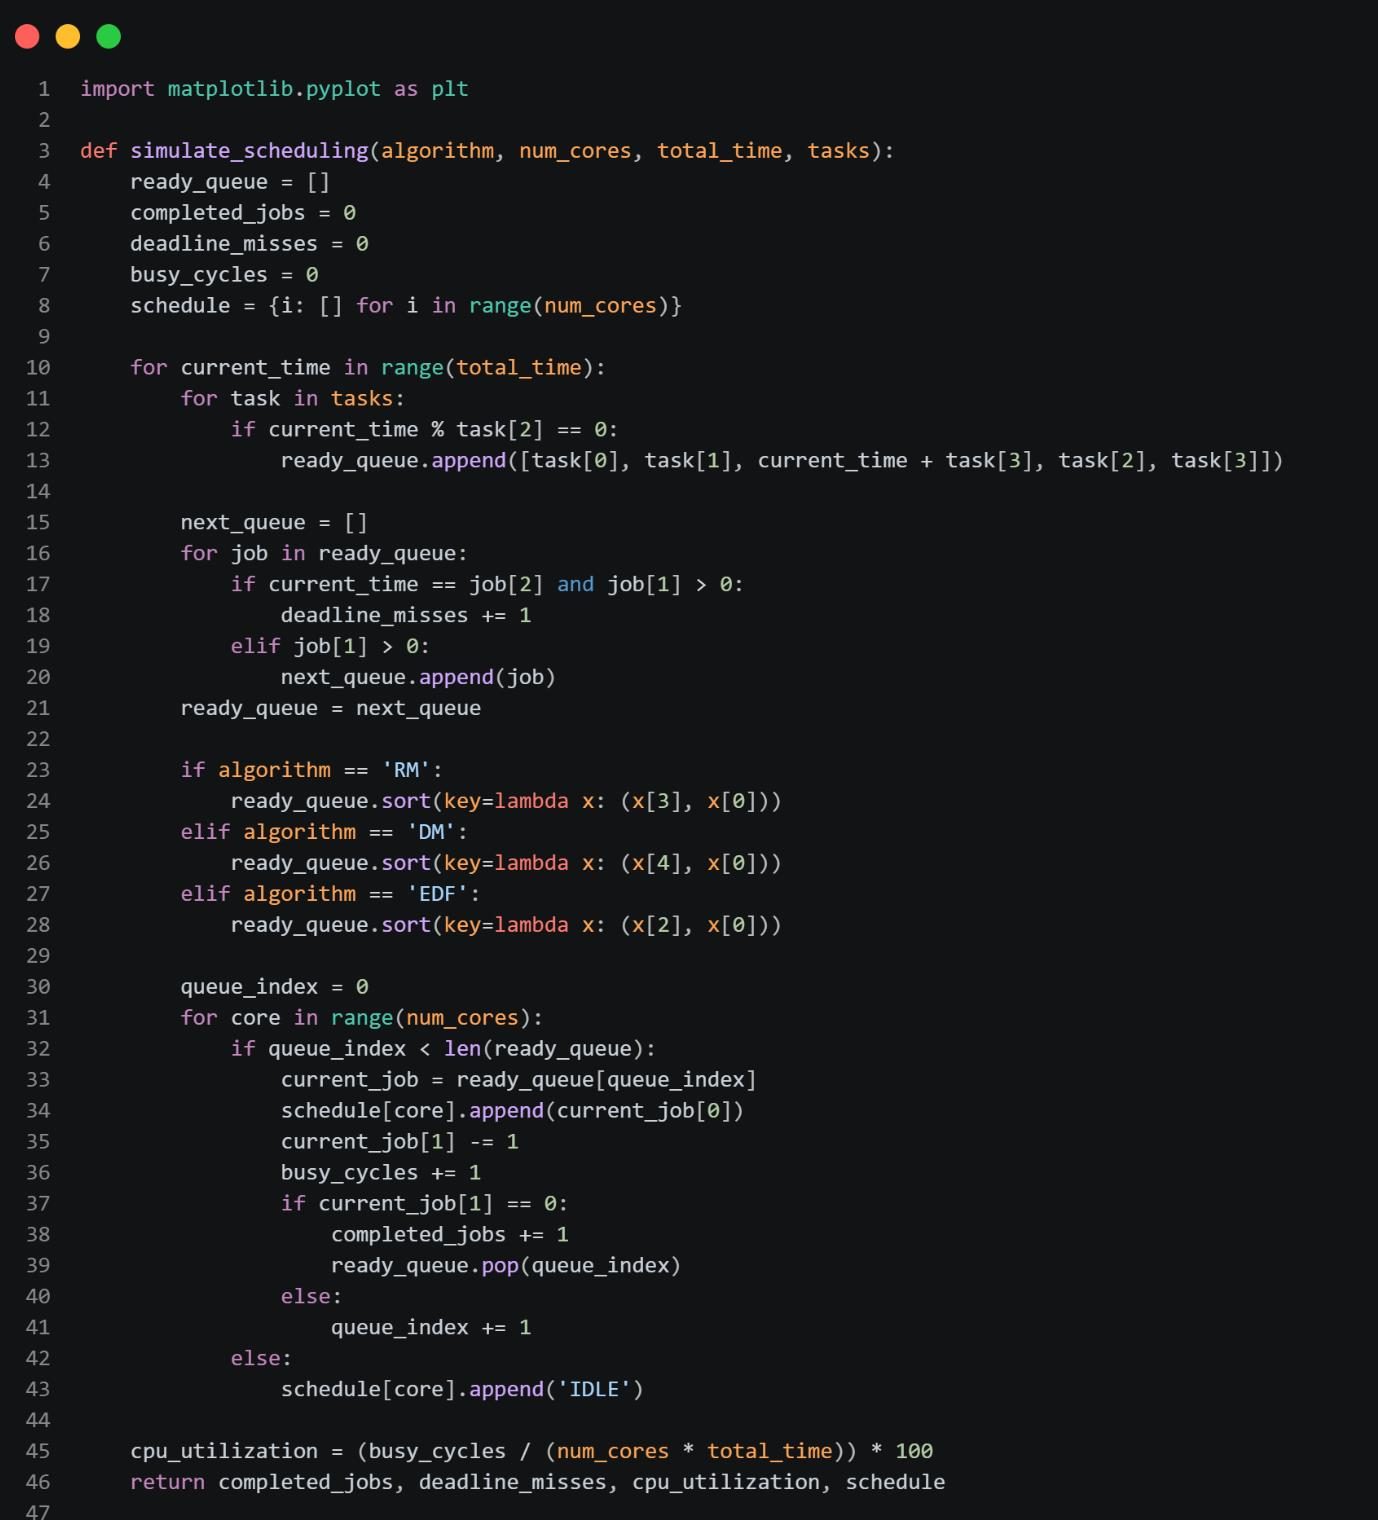
\includegraphics[width=\linewidth,height=.72\textheight,keepaspectratio]{assets/016_p010_02.png}\caption{Implementation and output: Simulator input and priority rules.}\label{fig:016_p010_020}\end{figure}
\begin{figure}[!htbp]\centering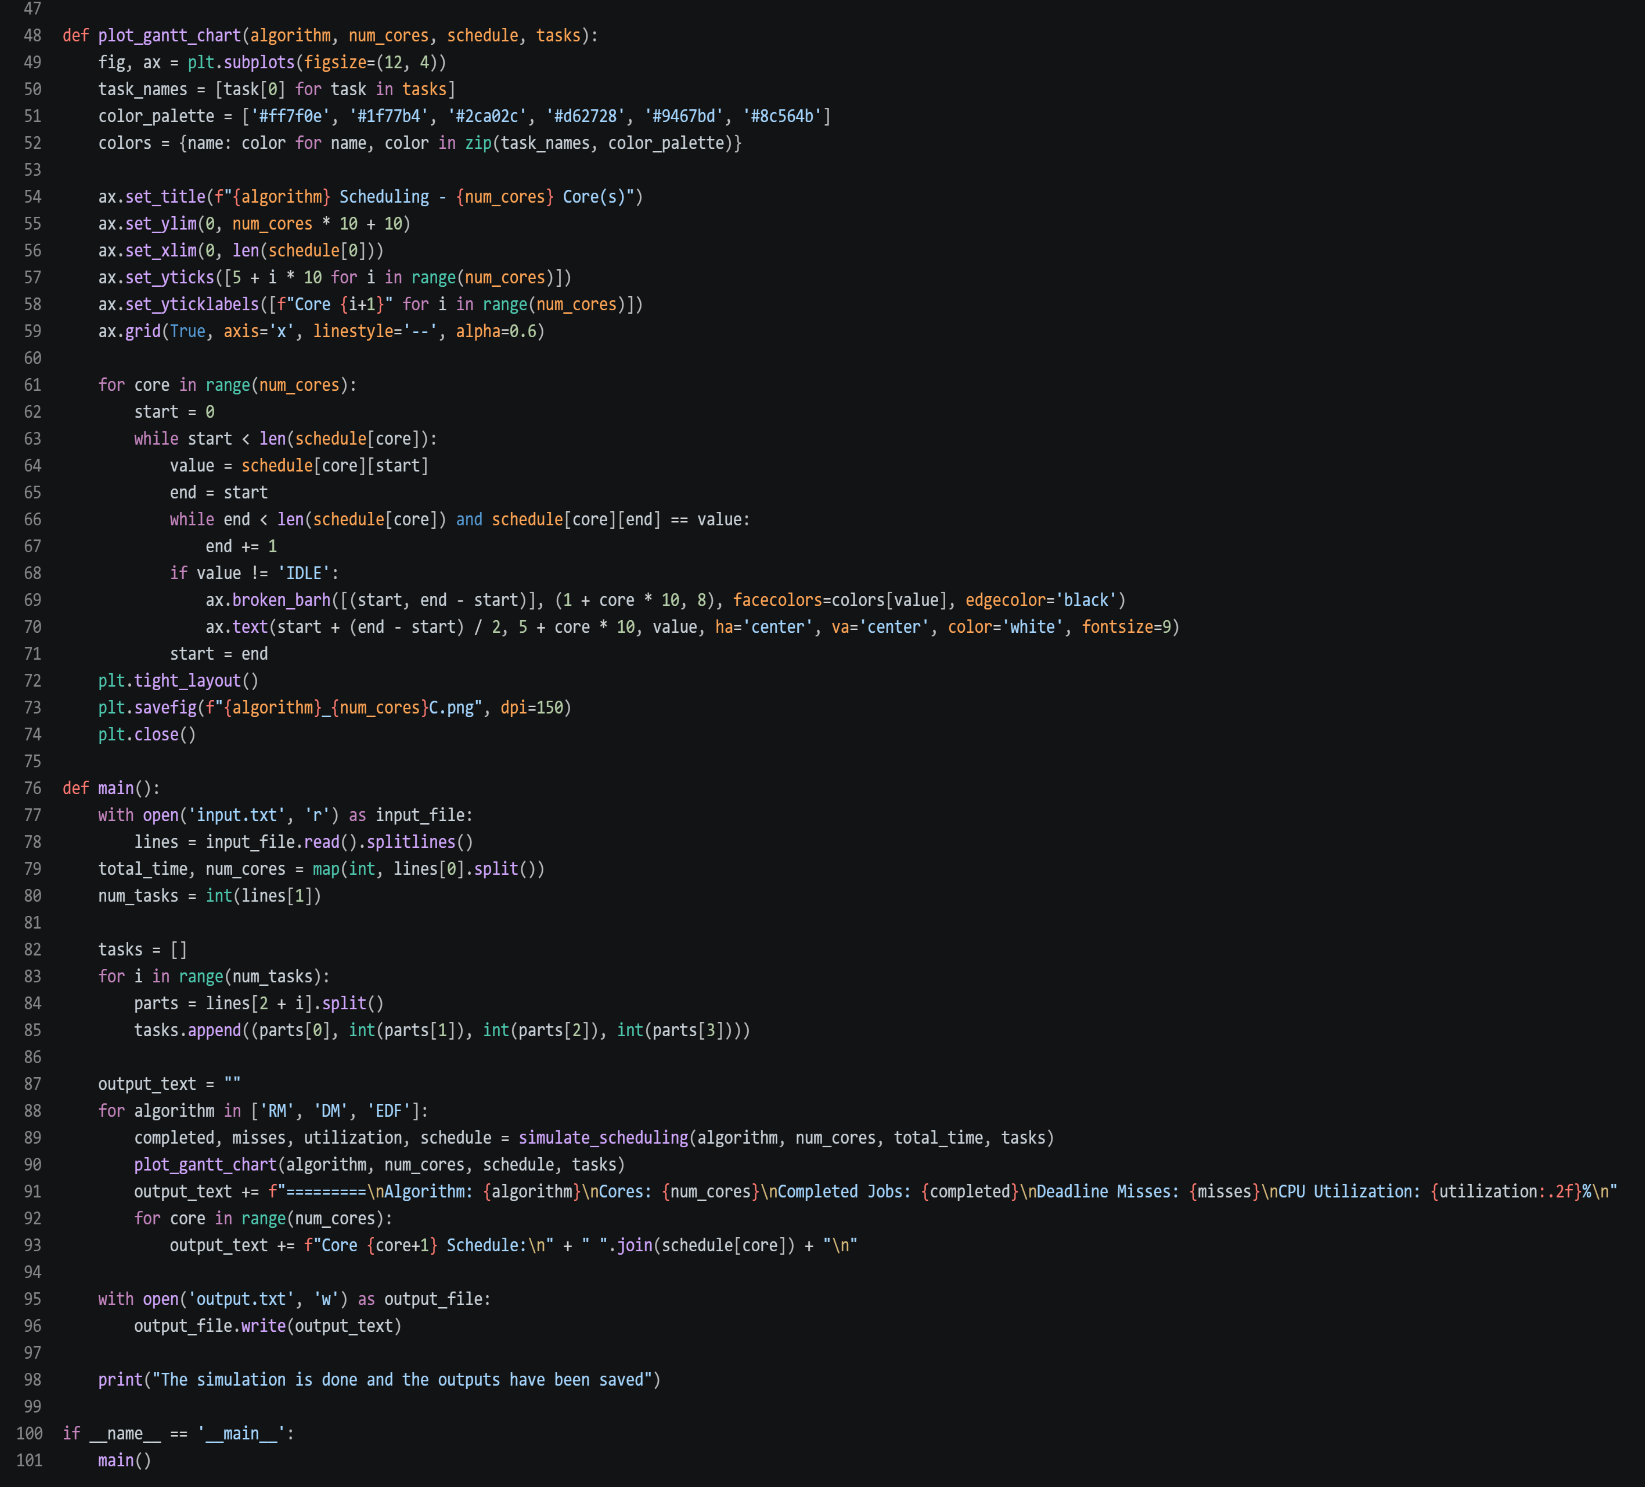
\includegraphics[width=\linewidth,height=.72\textheight,keepaspectratio]{assets/016_p011_01.png}\caption{Implementation and output: Simulator input and priority rules.}\label{fig:016_p011_010}\end{figure}
\clearpage
\section{Recorded one-core and two-core outcomes}

\begingroup\small\setlength{\tabcolsep}{3pt}\renewcommand{\arraystretch}{1.2}
\begin{longtable}{@{}p{0.1760\linewidth}p{0.1760\linewidth}p{0.1760\linewidth}p{0.1760\linewidth}p{0.1760\linewidth}@{}}
\toprule
\textbf{Policy} & \textbf{Cores} & \textbf{Completed jobs} & \textbf{Deadline misses} & \textbf{Utilization over recorded horizon} \\ \midrule
\endfirsthead
\textbf{Policy} & \textbf{Cores} & \textbf{Completed jobs} & \textbf{Deadline misses} & \textbf{Utilization over recorded horizon} \\ \midrule \endhead
RM & 1 & 17 & 0 & 83.33 percent \\
DM & 1 & 17 & 0 & 83.33 percent \\
EDF & 1 & 17 & 0 & 83.33 percent \\
RM & 2 & 17 & 0 & 41.67 percent \\
DM & 2 & 17 & 0 & 41.67 percent \\
EDF & 2 & 17 & 0 & 41.67 percent \\
\bottomrule\end{longtable}\endgroup

The run releases eight T1 jobs, four T2 jobs, and five T3 jobs:\allowbreak{} 17 jobs requiring 8+\allowbreak{}12+\allowbreak{}5=\allowbreak{}25 core-time units. Dividing by 30 yields 83.33 percent for one core, and dividing by 60 gives 41.67 percent averaged across two cores. This normalized utilization falls because capacity doubles;\allowbreak{} the supplied work does not halve. Aggregate periodic offered utilization is instead 1/\allowbreak{}4+\allowbreak{}3/\allowbreak{}8+\allowbreak{}1/\allowbreak{}7=\allowbreak{}43/\allowbreak{}56, approximately 76.79 percent. A finite horizon can differ from that long-run ratio.

\begin{figure}[!htbp]\centering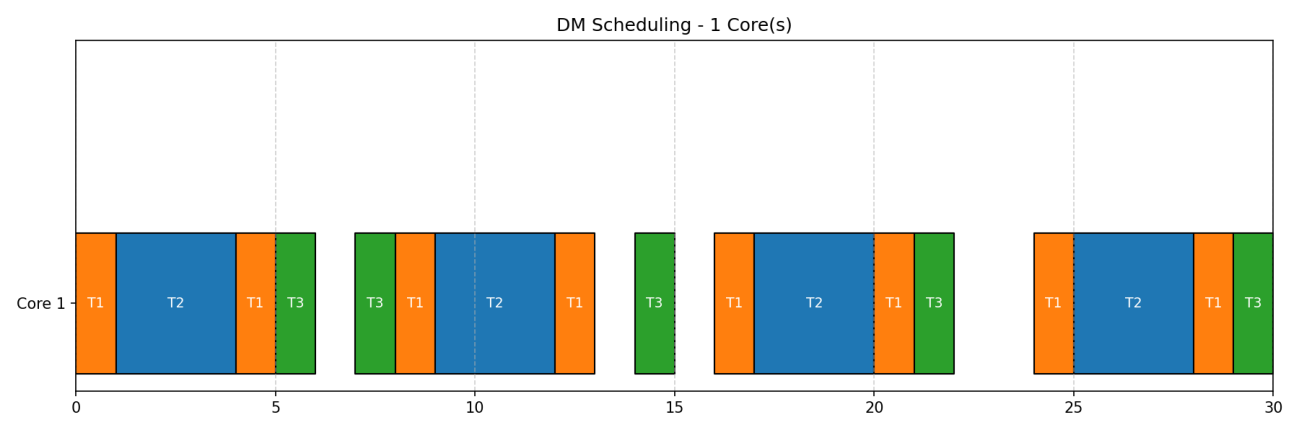
\includegraphics[width=\linewidth,height=.72\textheight,keepaspectratio]{assets/016_p013_01.png}\caption{Diagram or recorded result: Recorded one-core and two-core outcomes.}\label{fig:016_p013_010}\end{figure}
\begin{figure}[!htbp]\centering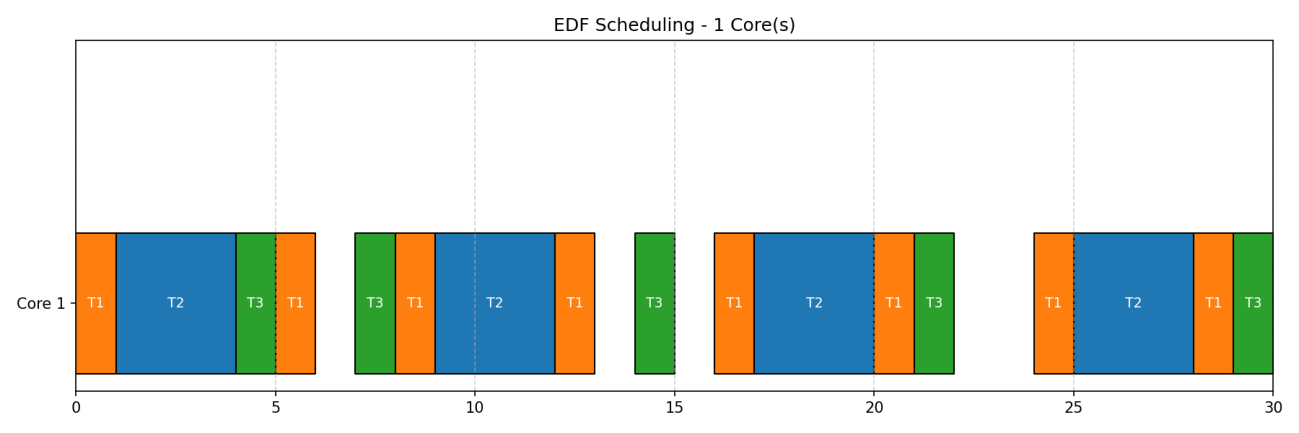
\includegraphics[width=\linewidth,height=.72\textheight,keepaspectratio]{assets/016_p014_01.png}\caption{Diagram or recorded result: Recorded one-core and two-core outcomes.}\label{fig:016_p014_010}\end{figure}
\begin{figure}[!htbp]\centering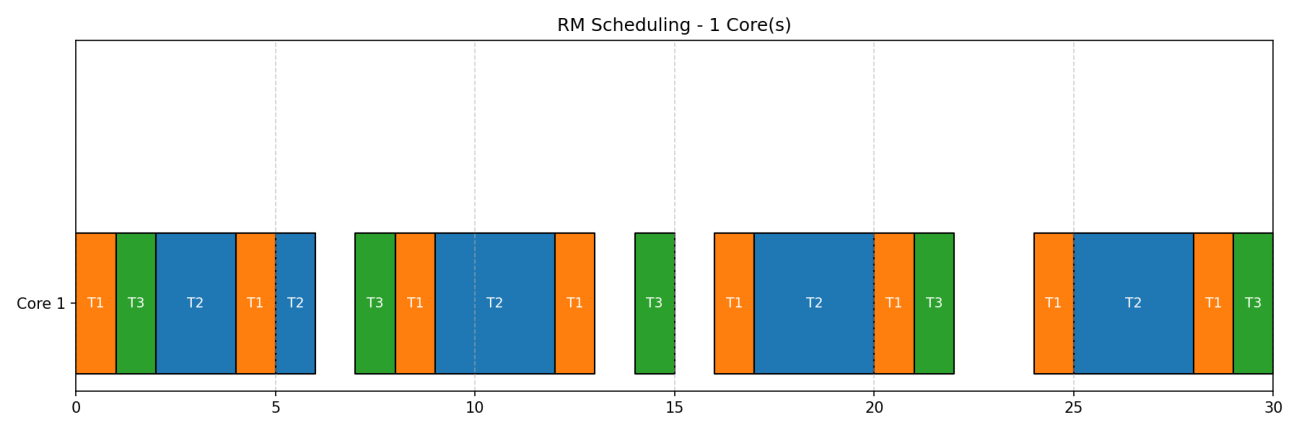
\includegraphics[width=\linewidth,height=.72\textheight,keepaspectratio]{assets/016_p014_02.png}\caption{Diagram or recorded result: Recorded one-core and two-core outcomes.}\label{fig:016_p014_020}\end{figure}
\begin{figure}[!htbp]\centering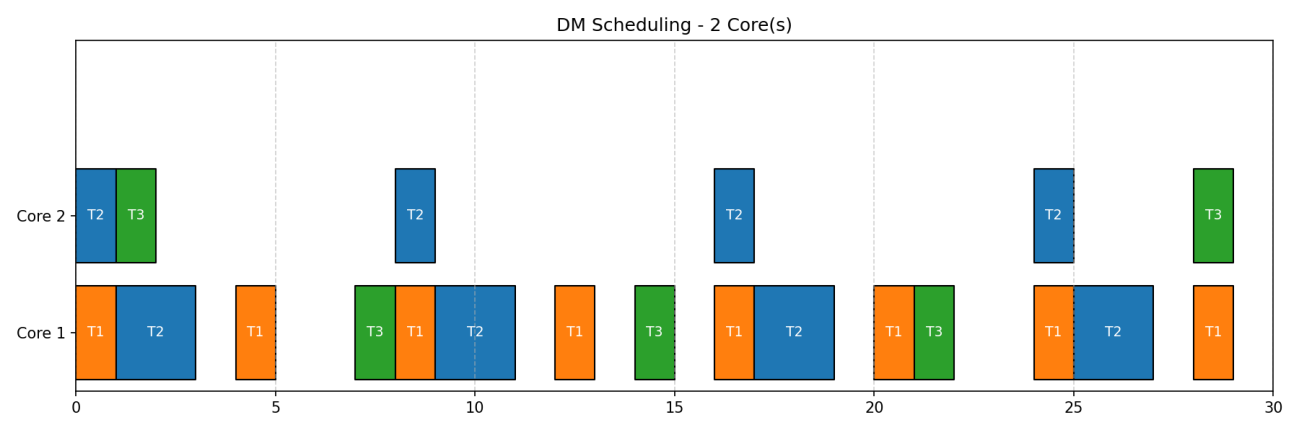
\includegraphics[width=\linewidth,height=.72\textheight,keepaspectratio]{assets/016_p017_01.png}\caption{Diagram or recorded result: Recorded one-core and two-core outcomes.}\label{fig:016_p017_010}\end{figure}
\begin{figure}[!htbp]\centering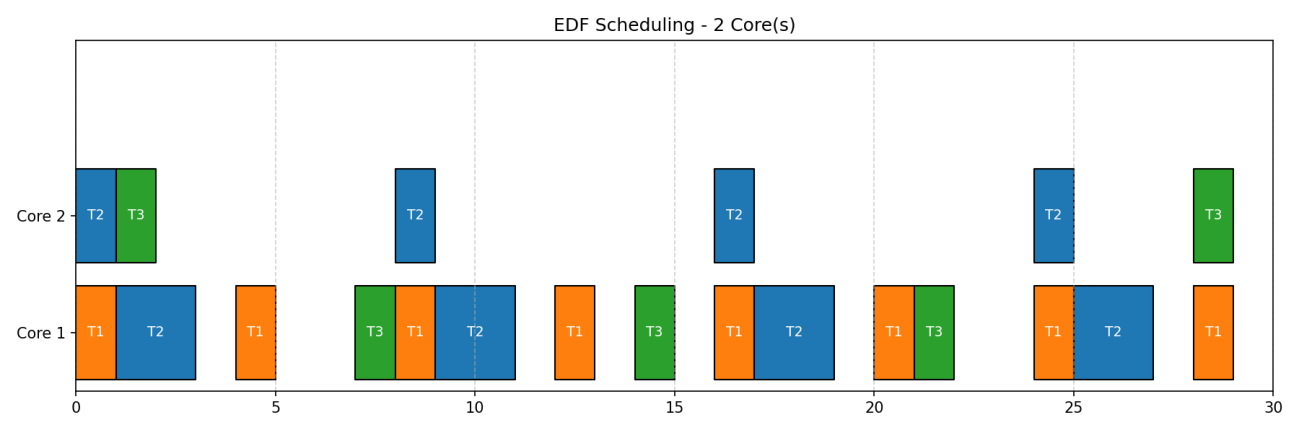
\includegraphics[width=\linewidth,height=.72\textheight,keepaspectratio]{assets/016_p017_02.png}\caption{Diagram or recorded result: Recorded one-core and two-core outcomes.}\label{fig:016_p017_020}\end{figure}
\begin{figure}[!htbp]\centering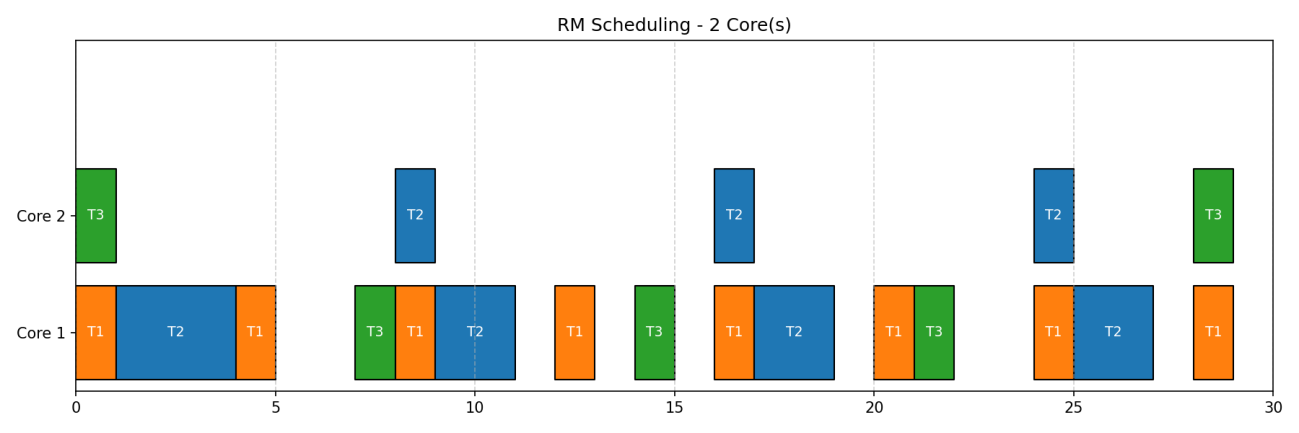
\includegraphics[width=\linewidth,height=.72\textheight,keepaspectratio]{assets/016_p018_01.png}\caption{Diagram or recorded result: Recorded one-core and two-core outcomes.}\label{fig:016_p018_010}\end{figure}
\clearpage
\section{Schedulability analysis}

RM and DM differ in their choice between T2 and T3, visible at the beginning of the one-core trace. Two cores permit jobs to overlap and add idle capacity, but deadline misses remain zero because the one-core run already completed every released job in the recorded interval. The EDF utilization guarantee applies to independent, preemptible periodic tasks with implicit deadlines under the stated execution assumptions. T2 has D<T, so the familiar implicit-deadline utilization-only test is insufficient here. Fixed-priority analysis requires an appropriate response-time test including interference and blocking assumptions;\allowbreak{} EDF requires a demand analysis for constrained deadlines. Zero misses in a 30-unit simulation do not prove indefinite schedulability. Similarly, the simulation does not measure power, so it cannot prove that one core is energy-optimal. The evidence supports a smaller hardware-capacity requirement for this observed workload and additional spare capacity with two cores.

\end{document}